\documentclass[a4paper, 12pt]{article}

\usepackage[left=2cm,right=2cm,
top=2cm,bottom=2cm,bindingoffset=0cm]{geometry}

\usepackage[T2A]{fontenc}
\usepackage[utf8]{inputenc}
\usepackage{color}
\usepackage{graphicx}
\usepackage{caption}
\usepackage{subcaption}
\usepackage{tikz}
\usepackage[english, russian]{babel}
\usepackage{ gensymb }
\usepackage{booktabs}
\usepackage{amsmath,amsfonts,amssymb,amsthm,mathtools}
\usepackage{lscape}
\usepackage{float}
\usepackage{pdflscape}
\usepackage{array}
\usepackage{multirow}
\usepackage{gensymb}

\begin{document}
		\begin{center}
		\textit{\textbf{Задача }}
	\end{center}
	
	К закрепленному в стене концу стержня $(x=0)$ подводится тепловой поток
	интенсивности q. На свободном конце стержня $(x=L)$ происходит конвективный
	теплообмен тепла. Коэффициент теплообмена $h$, температура окружающей среды $T_{cp}$.
	Через боковую поверхность стержня также происходит конвективный теплообмен.
	Площадь поперечного сечения стержня $S$ считается постоянной.
	
	Решить задачу методом конечных элементов с использованием одномерного
	линейного (симплекс) элемента. Выписать в тетради явное решение СЛАУ в случае
	когда стержень разбит на 3 элемента.
	
	Разбить стержень на 5 конечных элементов и вычислить температуру в узлах МКЭ
	запрограммировав на языке С++.
	
	Решить задачу при следующих данных:
	
	$k_x=75\left[\text{Вт/(см)}\cdot \celsius \right]$ - коэффициент теплопроводности материала, 
	
	$q=-150\left[\text{Вт/}\text{см}^2 \right]$ - считается, что положительное направление, когда тепло отводится от тела, так как по задаче тепло подводится, то знак минус
	
	$\alpha_g=10\left[\text{Вт/}\text{(см)}^2\cdot \celsius \right]$ - коэффициент теплообмена, $S=\pi \text{см}^2, L=7.5\text{ см}$
	

	\begin{figure}[h]
		\centering
		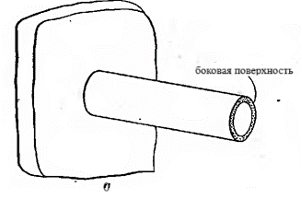
\includegraphics[width=0.5\textwidth]{pic.jpeg}
	\end{figure}
	
	\begin{center}
		\textbf{\textit{Решение}}
	\end{center}
	
	\textbf{1.} Дискретизация области одномерными элементами
	\begin{figure}[h]
		\centering
		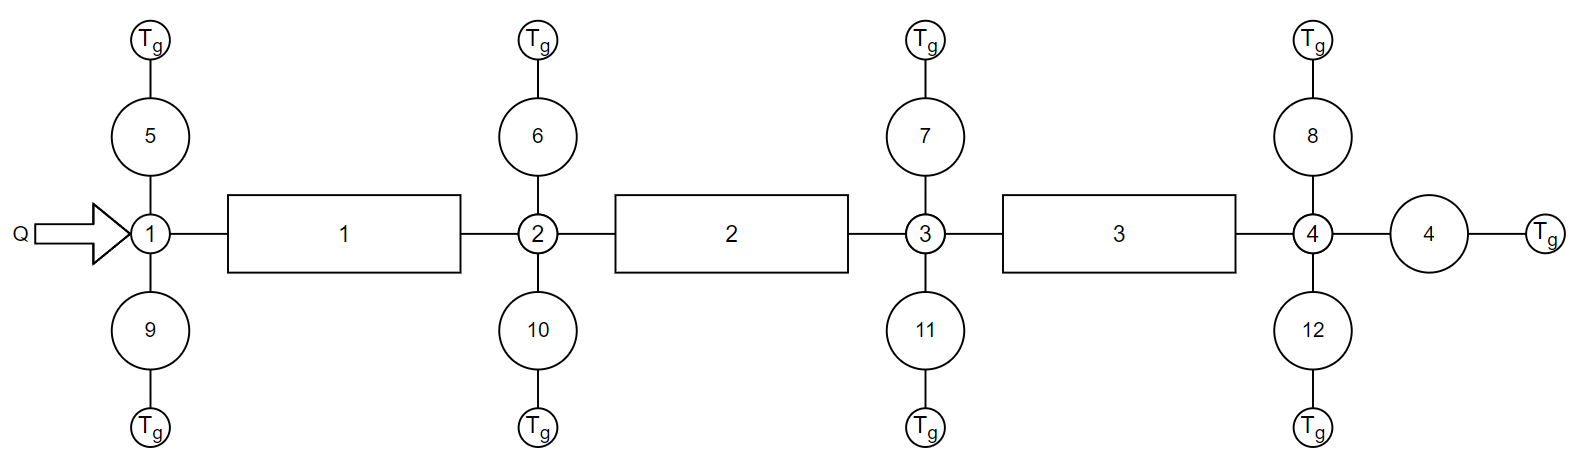
\includegraphics[width=1\textwidth]{image.png}
	\end{figure}
	
	Рассмотрим дифференциальное уравнение, описывающее распространение тепла в
	стержне: 
	\[
	-\frac{d}{dx}(k_x\frac{dT}{dx})=f \tag{1}
	\]

	где $f$ - погонная интенсивность подачи тепла, если внутри стержня есть источник. В задаче внутренние источники тепла не заданы, следовательно, $f=0$.
	
	Граничные условия:
	\[
	Q_1=k_x\frac{dT}{dx} \bigg{|}_{x=0} =-q; \qquad 	Q_2=k_x\frac{dT}{dx} \bigg{|}_{x=L} =\alpha_g(T_{cp}-T(l)) \qquad 	Q_2=k_x\frac{dT}{dx} \bigg{|}_{\Gamma} =\alpha_g(T_{cp}-T)
	\]

	Вариационная постановка: \\
	Так как нам дан стержень сечения $S$, то для решения задачи интегрирование надо проводить по объему стержня. Однако $V = S dx$, где $x$ — координата по длине стержня.
	\[
	\int\limits_0^L -\frac{d}{dx} \left( k_x \frac{dT}{dx} \right) S \delta T dx = 0, \, \delta T = \nu - \text{возможные изменения температуры} \, (\text{аналог невязки} \, \nu).
	\]
	
	Интегрируя выражение по частям, получим вариационную постановку:
	\[
	\int\limits_0^L -\frac{d}{dx} \left( k_x \frac{dT}{dx} \right) S \delta T dx = \left| 
	\begin{array}{cc}
		u= -k_x S  \delta T & du = -\dfrac{d \delta T}{dx} dx \vspace{0.1cm} \\
		dv=\dfrac{d}{d x}\left( \dfrac{d T}{d x}\right) dx & v = \dfrac{d T}{d x}
	\end{array} \right| = \]
	\[
	= -S \frac{d}{dx} \left( k_x \frac{dT}{dx} \right) \delta T \Big|_0^L + \int_0^L \left(k_x \frac{d T}{d x}\right) S \frac{d \delta T}{d x} d x = - F(\nu)+\int_0^L \left(k_x \frac{d T}{d x}\right) S \frac{d \delta T}{d x} d x.
	\]
	\[
	\int\limits_0^L -\frac{d}{dx} \left( k_x \frac{dT}{dx} \right) S dx - F(\nu) = 0.
	\]
	
	\[
	F(\nu) = S \frac{d}{dx} \left( k_x \frac{dT}{dx} \right) \delta T \Big|_0^L = S Q_2 \delta T_2 - S Q_1 \delta T_1
	\]
	
	Делим стержень на 3 элемента:
	\[
	\int\limits_{x_i}^{x_{i+1}} \frac{d\delta T}{dx} \left( k_x \frac{dT}{dx} \right) S dx -  t_1^{(i)} \delta T_i - t_2^{(i)}   \delta T_{i+1} = 0,\ i = 1, 2, 3
	\]

	
	
	
	
	
	
	
	
	
	
	
	
	
	
	
	
	
	
	
	Далее делим стержень на нужное количество элементов
	
	\[
	\int\limits_{x_i}^{x_{i+1}} \frac{d\delta T}{dx} \left( k_x \frac{dT}{dx} \right) S dx -  t_1^{(i)} \delta T_i - t_2^{(i)}   \delta T_{i+1} = 0
	\]
	
	Аппроксимируем линейно неизвестные функции
	
	\[
	T = N^{(i)} q^{(i)}, \, \delta T = N^{(i)} \delta q^{(i)}, \, N^{(i)} = \begin{bmatrix} N_1^{(i)} & N_2^{(i)} \end{bmatrix}, \, N_1^{(i)} = 1 - \frac{x - x_i}{x_{i+1} - x_i}, \, N_2^{(i)} = \frac{x - x_i}{x_{i+1} - x_i}
	\]
	
	\[
	q^{(i)} = \begin{bmatrix} T_i & T_{i+1} \end{bmatrix}, \, \delta q^{(i)} = \begin{bmatrix} \delta T_i & \delta T_{i+1} \end{bmatrix}
	\]
	
	Подставляем в интегральное уравнение и сводим решение к СЛАУ вида
	
	\[
 	t^{(i)}=K^{(i)}  q^{(i)} - P^{(i)}
	\]
	
	Суммируя по КЭ с учетом ГУ, получаем СЛАУ $K q = P$.
	
	
	
	
	
	
	
	
	
	
	
	
	
	
	
	
\end{document}